\section{Electric car sharing simulator}
\label{sec:Modelling}

Our goal is to study different design choices for electric car sharing systems. For this, we developed a flexible event-based simulator that allows us to compare different algorithms and tune their parameters while collecting metrics of interest. Simulations are based on the actual traces collected from operative FFCS providers in each city. This allows us to factor all spatial and temporal characteristics of actual FFCS customers habits.

\subsection{Simulation model}

We simulate a fleet of electric cars, which move in the city. Each car is characterized by its location, and the current status of battery charge.  The simulator takes as input a pre-recorded trace of rentals characterized by the start and end time, and initial and final geographic coordinates.

In more details, each trip $i \in \mathcal{I}$  is characterized by its start and end time, $t_{s}(i)$ and $t_{e}(i)$, and origin and destination coordinates, $o(i)$ and $d(i)$. For simplicity, we divide the city area into squared zones, of side 500\,m as before. We associate with each position one and only one zone $O(i)=zone(o(i))$ and $D(i)=zone(d(i))$. We assume a charging station $cs$, composed of $k$ poles, can be placed at the center of a given zone $z\in \mathcal{Z}$, so either $cs(z)=1$ if the station is present, or $cs(z)=0$ otherwise. $N=\sum_{z\in \mathcal{Z}}cs(z)$ is the total number of zones equipped with charging stations, with 
$K=N\cdot k$ the total number of poles.


We have a set $\mathcal{A}$ of cars, with its cardinality $\left\vert{\mathcal{A}}\right\vert$ obtained by the trace. Each car $a\in \mathcal{A}$ at time $t$ is characterized by its position $p(a,t)$, its zone $P(a,t)=zone(p(a,t))$, and the residual battery capacity $c(a,t)\in[0,C]$, with $C$ being the maximum nominal capacity.

The simulator processes each rental event $i$ in temporal order. 
When a \emph{rental-start} event $i$ is processed at time $t=t_{s}(i)$, we choose randomly one of the most charged  available car in the closest zones to the initial position zone $O(i)$. In formulas, we get a car $\bar{a} \in \mathcal{A}$ such that:
\[
c(\bar{a},t) \geq c(\hat{a},t)\ \forall \hat{a} \in \argmin_{a \in A} {dist(O(i), P(a,t))}.
\]
Basically, we mimic the normal behavior of FFCS customers that use their smartphone to rent the closest car from their position and are worried about vehicle range~\cite{RangeAnxiety}. Notice that this behavior is
independent from whether the car is at a pole being charged or not.




A \emph{rental-end} event is then scheduled using the trace final time $t_{e}(i)$ and desired destination location $d(i)$.

When a \emph{rental-start} event $i$ is processed at time $t=t_{s}(i)$, we look for a car in the initial position zone $O(i)$. If one or more cars are present, we select (one among) the most charged car, i.e, get the car $a\in \mathcal{A}$ such that
\[
P(a,t) = O(i) \, \land \, c(a,t) \geq c(a',t)\ \forall a'\mid P(a',t) = O(i),
\]
independently whether the car is at a pole being charged or not.\footnote{We choose this policy because people are worried about vehicle range~\cite{RangeAnxiety}.}


% %However, this hypothesis helps the charging stations to be emptied when cars are charged: for a more realistic approach, real user behavour should be better evaluate in future work.
If no car is present, we select the closest zone to $O(i)$ containing an available car, mimicking the normal behavior of FFCS customers that use their smartphone to rent the closest car from their position.
A \emph{rental-end} event is then scheduled using the trace final time $t_{e}(i)$ and location $d(i)$.

When car $a$ rental-end event is processed at time $t_{e}(i)$, we return the car in a real position $p(a,t_{e}(i))$, chosen according to the behavior described in Section \ref{subsec:policies}. The simulator updates the battery charge status by consuming an amount of energy proportional to the real trip distance:
\begin{eqnarray*}
	&& c(a,t_{e}(i)) = \nonumber
	 \\
	&& \hspace{0cm}   \max{(c(a,t_{s}(i)) - Energy(p(a,t_{s}(i)), p(a,t_{e}(i))), 0)} 
\end{eqnarray*}

%\[
%c(a,t_{e}(i)) = \max{(c(a,t_{s}(i)) - Energy(p(a,t_{s}(i)), p(a,t_{e}(i))), 0)}
%\]
with $Energy(\cdot)$ that models the energy consumed to go from the car origin $p(a,t_{s}(i))$ to the car destination $p(a,t_{e}(i))$.
In case $c(a,t_{e}(i)) = 0$, the trip $i$ is declared {\it infeasible}. 
The discharged car $a$ still performs further trips, all marked as infeasible, until it reaches a charging station.

\subsection{Car charging policies}
\label{subsec:policies}

When returning the car, the customer may connect the car to a pole in a station, hence charging the car battery and possibly deviating the real destination from the desired one.

In this Section, we define different policies that the electric FFCS may enforce, and different probabilistic behaviors of customers. 
We investigate the following policies:
\begin{itemize}
 	\item{\it Free Floating}: the customer must connect the car to a charging pole if and only if it is available in the desired final zone $D(i)$;
 	\item{\it Forced}: cars must be connected to a pole when the percentage of battery charge at the end of the rental $i$ would go below a certain threshold $\pi$, i.e., $(c(a,t_{s}(i)) - Energy(p(a,t_{s}(i)), d(i))) \cdot 100/ C\leq  \pi $. This implies the customer can be \textit{rerouted} to the closest zone to the desired one $d(i)$, if no free pole exists in the zone; %Battery consumption takes into account the additional traveled distance.
 	\item{\it Hybrid}: the customers follow the forced policy; they may  also choose to connect to a charging pole available in the desired ending zone $D(i)$ with probability $w\in [0,1]$;
 %if the $c(a,t)\leq\pi$, cars must be returned to the closest recharging zone to $d(i)$.
\end{itemize}

The \textit{Free Floating} policy never obliges the customer to bring the car far from the desired ending location, even in case battery is close to exhaustion.
\textit{Forced} mandates to connect cars to a charge station only when energy runs low, thus trying to protect from battery exhaustion.
\textit{Hybrid} balances the two policies, with $w$ that measures the level of customers willingness to collaborate. $w=0$ is equivalent to the Forced policy, while $w=1$ adds to the Forced policy the Free Floating policy,  thus always connecting the car to a charging pole if available in their final position zone.

\subsection{Charging stations placement}

Given a number of charging station $N$, our first objective is to place them in the city area so to let all rentals feasible, i.e., to find a charging stations placement so that
\[
c(a,t_e(i))>0\ \forall a \in \mathcal{A}, \forall  i \in \mathcal{I}
\]
Since we do not make any assumption on the set of trips $\mathcal{I}$, we cannot know a-priori if a solution exists and provide an analytical general solution. Moreover the number of candidate solutions increases as the binomial coefficient ${\left\vert{\mathcal{Z}}\right\vert}\choose\ N$, making ineffective to numerically compute all possibilities. Instead, we will provide a class of greedy algorithms and analyze the performance in our specific cases of $\mathcal{I}$.
In details, each zone $z\in\mathcal{Z}$ is assigned a likelihood $l_z \geq 0$.
We then solve the problem of finding the subset of $N$ zones that maximizes the total likelihood. In formulas, 
$$\max \sum_{z\in\mathcal{Z}} cs(z)l_z$$

subject to:
$$\sum_{z\in\mathcal{Z}} cs(z) = N$$
$$cs(z)\in \{0,1\},  \forall z \in \mathcal{Z}$$

The above optimization problem can be solved by greedily choosing the top $N$ zones, ordered in decreasing likelihood. We compare the performance of different placement algorithms based on different definition of the likelihood.
\begin{itemize}
  \item{\it Random placement}: $l_z$ is an independent and identical distributed random uniform variable, so that charging stations result placed at random;
  \item{\it Average parking time}: $l_z$ is the average parking duration in $z$ as recorded in the trace;
  \item{\it Total number of parkings}: $l_z$ is the total number of parking events recorded in $z$ in the trace;
  \item{\it Total parking time}: $l_z$ is the total parking time accumulated in $z$ by all cars recorded in the trace. In each zone, it is the product of the two previous metrics.
\end{itemize}
As discussed in Section~\ref{sec:dataspace}, the last three heuristics are driven by the intuition that placing charging stations in those zones where cars are parked for long time (average parking time) or frequently parked (total number of parkings) could improve system performance.

\begin{figure*}[t!]
    \begin{center}
       
\includegraphics[width=0.49\textwidth]{figures/legenda2.pdf}
    \end{center}
    \begin{center}
        \begin{subfigure}{0.49\textwidth}
            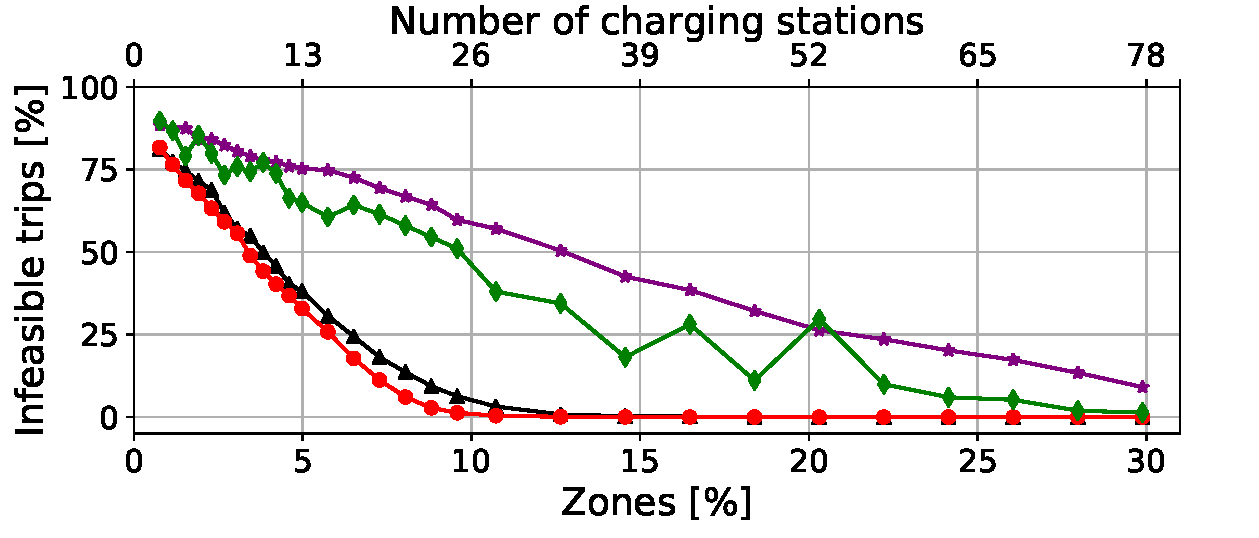
\includegraphics[width=\columnwidth]{figures/Torino_zonesVsDeaths_algorithms_acs-4_tt-25_policy-FreeFloating.pdf}
            \caption{Turin}
            \label{fig:zone_vs_deaths_torino}
        \end{subfigure}
         \begin{subfigure}{0.49\textwidth}
             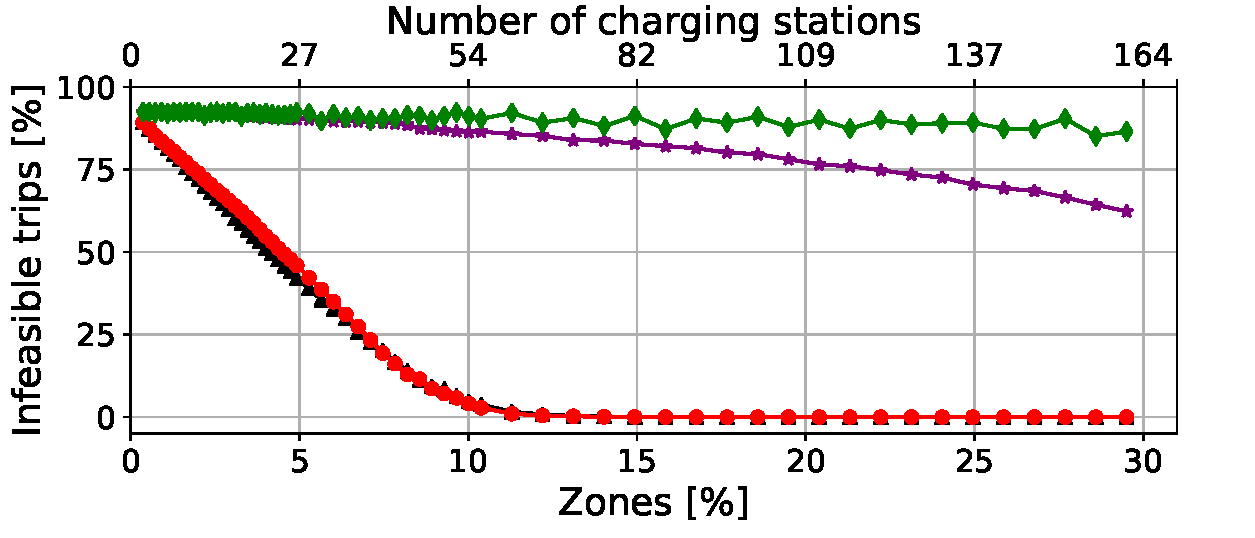
\includegraphics[width=\columnwidth]{figures/Milano_zonesVsDeaths_algorithms_acs-4_tt-25_policy-FreeFloating.pdf}
             \caption{Milan}
             \label{fig:zone_vs_deaths_milano}
         \end{subfigure}
         \begin{subfigure}{0.49\textwidth}
             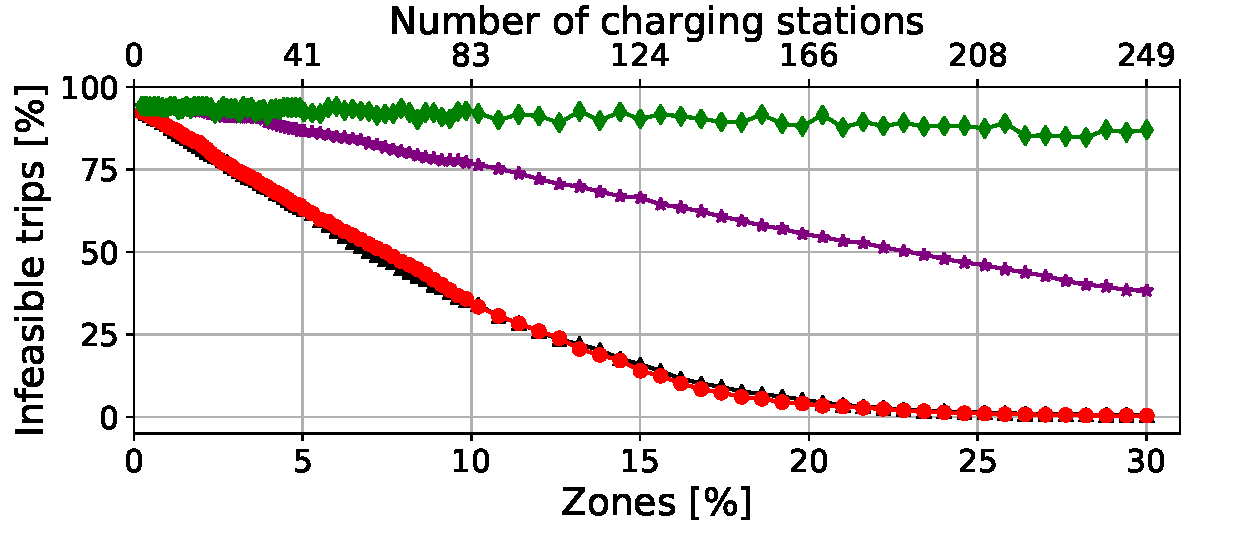
\includegraphics[width=\columnwidth]{figures/Berlino_zonesVsDeaths_algorithms_acs-4_tt-25_policy-FreeFloating.pdf}
             \caption{Berlin}
             \label{fig:zone_vs_deaths_berlino}
         \end{subfigure}
         \begin{subfigure}{0.49\textwidth}
             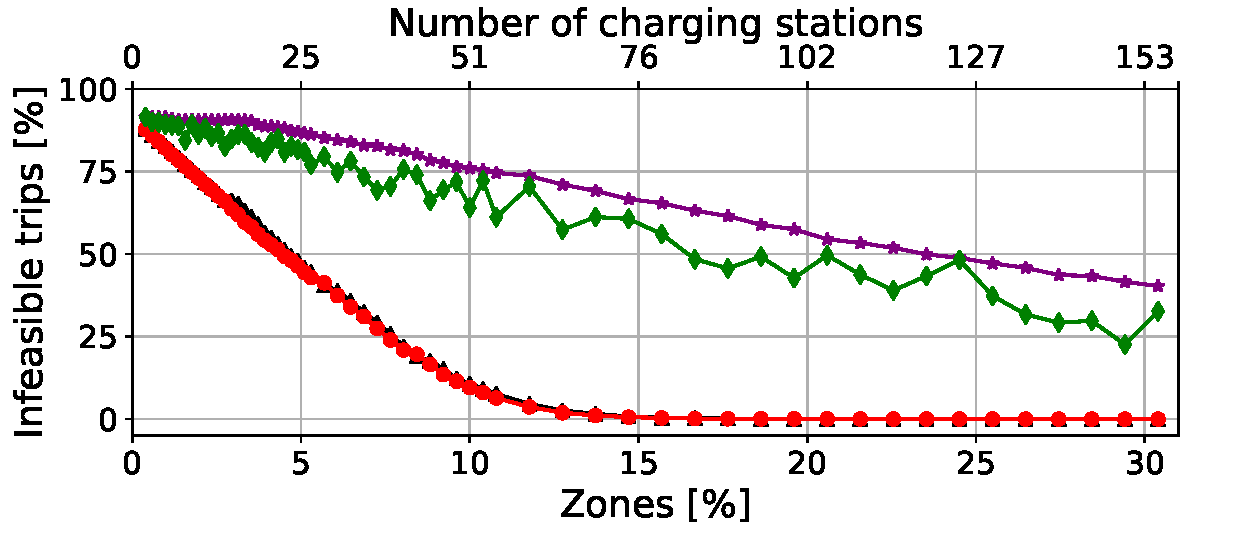
\includegraphics[width=\columnwidth]{figures/Vancouver_zonesVsDeaths_algorithms_acs-4_tt-25_policy-FreeFloating.pdf}
             \caption{Vancouver}
             \label{fig:zone_vs_deaths_vancouver}
         \end{subfigure}         
 	\caption{Percentage of unfeasible trips as function of charging station number, for different placement algorithms and city. Placing charging stations where cars are frequently parked is much better than where cars stay parked for long time.}
         \label{fig:deathsVsZones_algorithm}
\end{center}
\end{figure*}

\subsection{Performance metrics and parameters}

The simulator measures metrics that are  key to assess in the quality of experience for the customers:
\begin{itemize}
 	\item \emph{Infeasible trip}: measures if a trip $i$ performed by a car $a$ ends with a completely discharged battery, i.e., when $c(a,t_{e}(i))= 0$;
 	\item \emph{Charge event}: indicates a trip $i$ that ends with putting in charge the car, implying the burden to drive to the pole position, and plug the car;
 	\item \emph{Reroute event}: a trip $i$ where the customer is rerouted to a zone different from the  desired destination because forced to charge the car $a$, i.e., $P(a,t_{e}(i))\neq D(i)$;
 	\item \emph{Walk distance}: distance between the desired final location $d(i)$ and the actual final position $p(a,t_{end}(i))$.
 \end{itemize}

The number of infeasible trips are critical, and the system shall be engineered so that they never happen. Other performance metrics shall be minimized. 
In addition to the above metrics, the simulator collects statistics about car battery charge level $c(a,t)$, and fraction of time a battery stays under charge.

\subsection{Simulation scenario}

We focus on key design parameters, i.e., the charging station placement and return policies.
We then study the impact on the number of zones that are equipped with charging stations $N$, and the number of poles $k$ of each charging station.

Table~\ref{tab:summary} summarizes the dataset main characteristics.
We consider in each city a fleet that has a number of cars equal to the one observed in the trace. Electric cars have the same nominal characteristics as the Smart ForTwo Electric Drive, i.e., $17.6\,kWh$ battery, for $135\,km$ of range, with a discharge curve $Energy()$ that is proportional to the traveled distance ($12.9\,kWh/100\,km$). \footnote{\url{https://www.smart.com/uk/en/index/smart-electric-drive.html}} 
Charging stations have $k=4$ low power ($2\,kW$) poles each. These are cheap to install and a good compromise between costs, power requested, and occupied road section. We model a simple linear charge profile (complete charge in 8 hours and 50 minutes in our case). At last, the initial car position, only affecting the simulation transient, is chosen randomly.

Our simulator, written in Python, takes less then 5 seconds to complete a single simulation for a given city and parameter set. 
Due to the large number of simulations, we run them in parallel.
Each simulation produces 100\,MB of detailed logs, that we process on a Big Data cluster of 30 nodes using PySpark.%\footnote{\url{http://spark.apache.org/docs/latest/api/python/\#}}.
